\chapter{Universal and Modular Jastrow Factors for the Transcorrelated Method}
\label{chap:universal}

The contents of this chapter are planned to be expanded for a future publication. Some contents may be repeated there.

\section{Introduction}

So far, the \gls{TC} methods we have discussed had one major bottleneck in common: the optimisation of the Jastrow factor. While VMC in itself does not scale unfavourably, the fact that we need so many VMC cycles in order to properly optimise for TC (see \autoref{chap:opt}) results in a significant computational cost. For large systems, this can become the prohibitive step in the workflow.

Here we explore some alternative avenues to construct Jastrow factors for use in the transcorrelated method. In particular, we consider constructing ``universal'' Jastrow factors that do not need any optimisation. These have already been introduced in the literature,\supercite{fournaisNonIsotropic2007,fournaisSharp2005,tewSecond2008,szenesStriking2024} and are constructed to satisfy cusp conditions. We will also construct Jastrow factors from those optimised for atomic systems. That is, we optimise the Jastrow factor for the atom, and use the same Jastrow factor for molecules (so that the molecular Jastrow is the sum of atomic Jastrows). In effect, this would allow us to compile sophisticated atomic Jastrow factors that may be stored in a database for easy retrieval when considering larger systems, without any optimisation. We also consider keeping some components of these Jastrows fixed, while optimising other elements as a ``molecular correction'' to the atomic Jastrow factor.

These updated workflows represent significant improvements in the scalability and ease of use for TC methods, while arguably being more conceptually satisfying by making the Jastrow factors more general.

\section{Theory}

In this chapter, we study various choices of Jastrow factors to avoid the need for lengthy optimisation. These may be divided into two broad categories: universal Jastrow factors and atomic Jastrow factors.

\subsection{Universal Jastrow Factors}

A universal form for the Jastrow factor has already been presented by Fournais \emph{et al} in 2005,\supercite{fournaisSharp2005} and has occasionally made further appearances in the literature.\supercite{tewSecond2008,szenesStriking2024} The key advantage to using these is that we require no optimisation at all, while key disadvantages are that we must be careful about cut off functions, and we do not have as much flexibility so we cannot tailor the Jastrow factor to e.g. excited states.

The universal form of the Jastrow, which we shall dub the ``Fournais-Jastrow'' factor is given by\supercite{fournaisSharp2005,fournaisNonIsotropic2007}
\begin{equation}
    \label{eq:fournais-full}
    J = -\sum_I\sum_i Z_Ir_{iI} + \frac 12\sum_{i<j}r_{ij} + \frac{2-\pi}{6\pi}\sum_I\sum_{i<j}Z_I\bm r_{iI}\cdot \bm r_{jI}\ln(r_{iI}^2+r_{jI}^2),
\end{equation}
where, as usual, upper case indices denote the nucleus, and lower case indices represent electrons. The first term resolves the electron-nucleus cusps, the second term resolves the electron-electron cusps, and finally the last term resolves electron-electron-nucleus cusps. However, these terms are unbounded, and indeed are valid only close to coalescence points. For this reason, we introduce cutoff functions on each term.

Using the form of the cutoff functions used in previous chapters, that is $t(r,L) = (1-r/L)^3\Theta(r-L)$, we find unreasonable energies even for extremely small cutoffs. For example, with this form of cutoff with the electron-nucleus and electron-electron terms, and $L=0.1$ Bohr, we get a reference energy of $-246.604$ for N$_2$ with the \avtz basis set, whereas the \gls{HEAT} result is known to be $-109.5425$.\supercite{fellerSurvey2008}.

Thus, we instead use gaussian cutoffs, which are smooth but still decay rapidly. Our Jastrow factor therefore becomes
\begin{align}
    \label{eq:fournais-full-cutoffs}
    J &= -\sum_I\sum_i Z_Ir_{iI}\e^{-r_{iI}^2/L_{ee}^2} + \frac 12\sum_{i<j}r_{ij}\e^{-r_{ij}^2/L_{en}^2} \nonumber \\
    &\quad + \frac{2-\pi}{6\pi}\sum_I\sum_{i<j}Z_I\bm r_{iI}\cdot \bm r_{jI}\ln(r_{iI}^2+r_{jI}^2)\e^{-r_{iI}^2/L_{een}^2}\e^{-r_{jI}^2/L_{een}^2},
\end{align}
where $L_{ee}, L_{en}, L_{een}$ are cutoff parameters. For this study, we take $L\mathdef L_{ee} = L_{en} = L_{een}$, and consider three variants of equation \ref{eq:fournais-full-cutoffs}:
\begin{itemize}
    \item The full Fournais-Jastrow factor, as in equation \ref{eq:fournais-full-cutoffs}.
    \item Neglecting the electron-electron-nucleus term and resolving the electron-nucleus cusp using the approach described in \autoref{chap:opt} (instead of via the $r_{iI}$ terms), which is known to be a better way of handling electron-nucleus cusps.\supercite{drummondJastrow2004,needsVariational2020} We'll dub this the $ee+en$-Jastrow.
    \item Neglecting both the electron-electron-nucleus and electron-nucleus terms. This has already been studied in the context of TC-DMRG,\supercite{szenesStriking2024} though the choice of cutoffs may result in uncontrollably nonvariational energies. This is the simplest form, containing only $r_{ij}$ terms, and we dub it the ``$ee$-Jastrow''.
\end{itemize}

Consider again the nitrogen molecule at equilibrium. We treat the result from \gls{HEAT}\supercite{fellerSurvey2008} as the exact nonrelativistic ground state energy, and so this is as a lower bound for the lowest eigenvalue of $\htc$ for the various Jastrow factors. For each of the three choices above, there is only one parameter, $L$. For the Fournais-Jastrow factor, we find that the reference xTC-energy with a cutoff of $L=0.1$ Bohr at \avtz is $-115.122$ Hartree, which is below the HEAT result. This may be due to numerical issues from the complexity of this Jastrow factor form. Since this is such a small cutoff, the TC and non-TC energies should be roughly equal. For simplicity, we exclude the Fournais-Jastrow factor from this study and consider the $ee$- and $ee+en$-Jastrow factors.

The energy of the N$_2$ molecule and N atom with the \avtz basis set for the $ee$- and $ee+en$-Jastrow factors are shown in figure \ref{fig:fournais-cutoff-n2}. Shown are three non-TC energies: the non-TC (RHF) reference energy, the non-TC-FCIQMC energy, and the HEAT (effectively \gls{CBS} energy). Plotted as a function of $L$ are three TC energies, the xTC (RHF) reference energy, the xTC-MP2 energy, and the xTC-FCIQMC energy. For small $L$, we expect the non-TC and xTC reference and FCIQMC energies to coincide, which they approximately do. In contrast, for large $L$ we expect the energies to become unstable, as we start to include spurious long-range correlation. However, it is worth noting that according to these plots, ``long-range'' is already at $\approx 0.4$ Bohr, as the energies are all below the HEAT result. In every case, $L=0.3$ Bohr is shown to energies above that of HEAT but below that of non-TC. We therefore use $L=0.3$ Bohr as our ``universal'' cutoff for these Jastrows factors.

\begin{figure}[htbp]
    \centering
    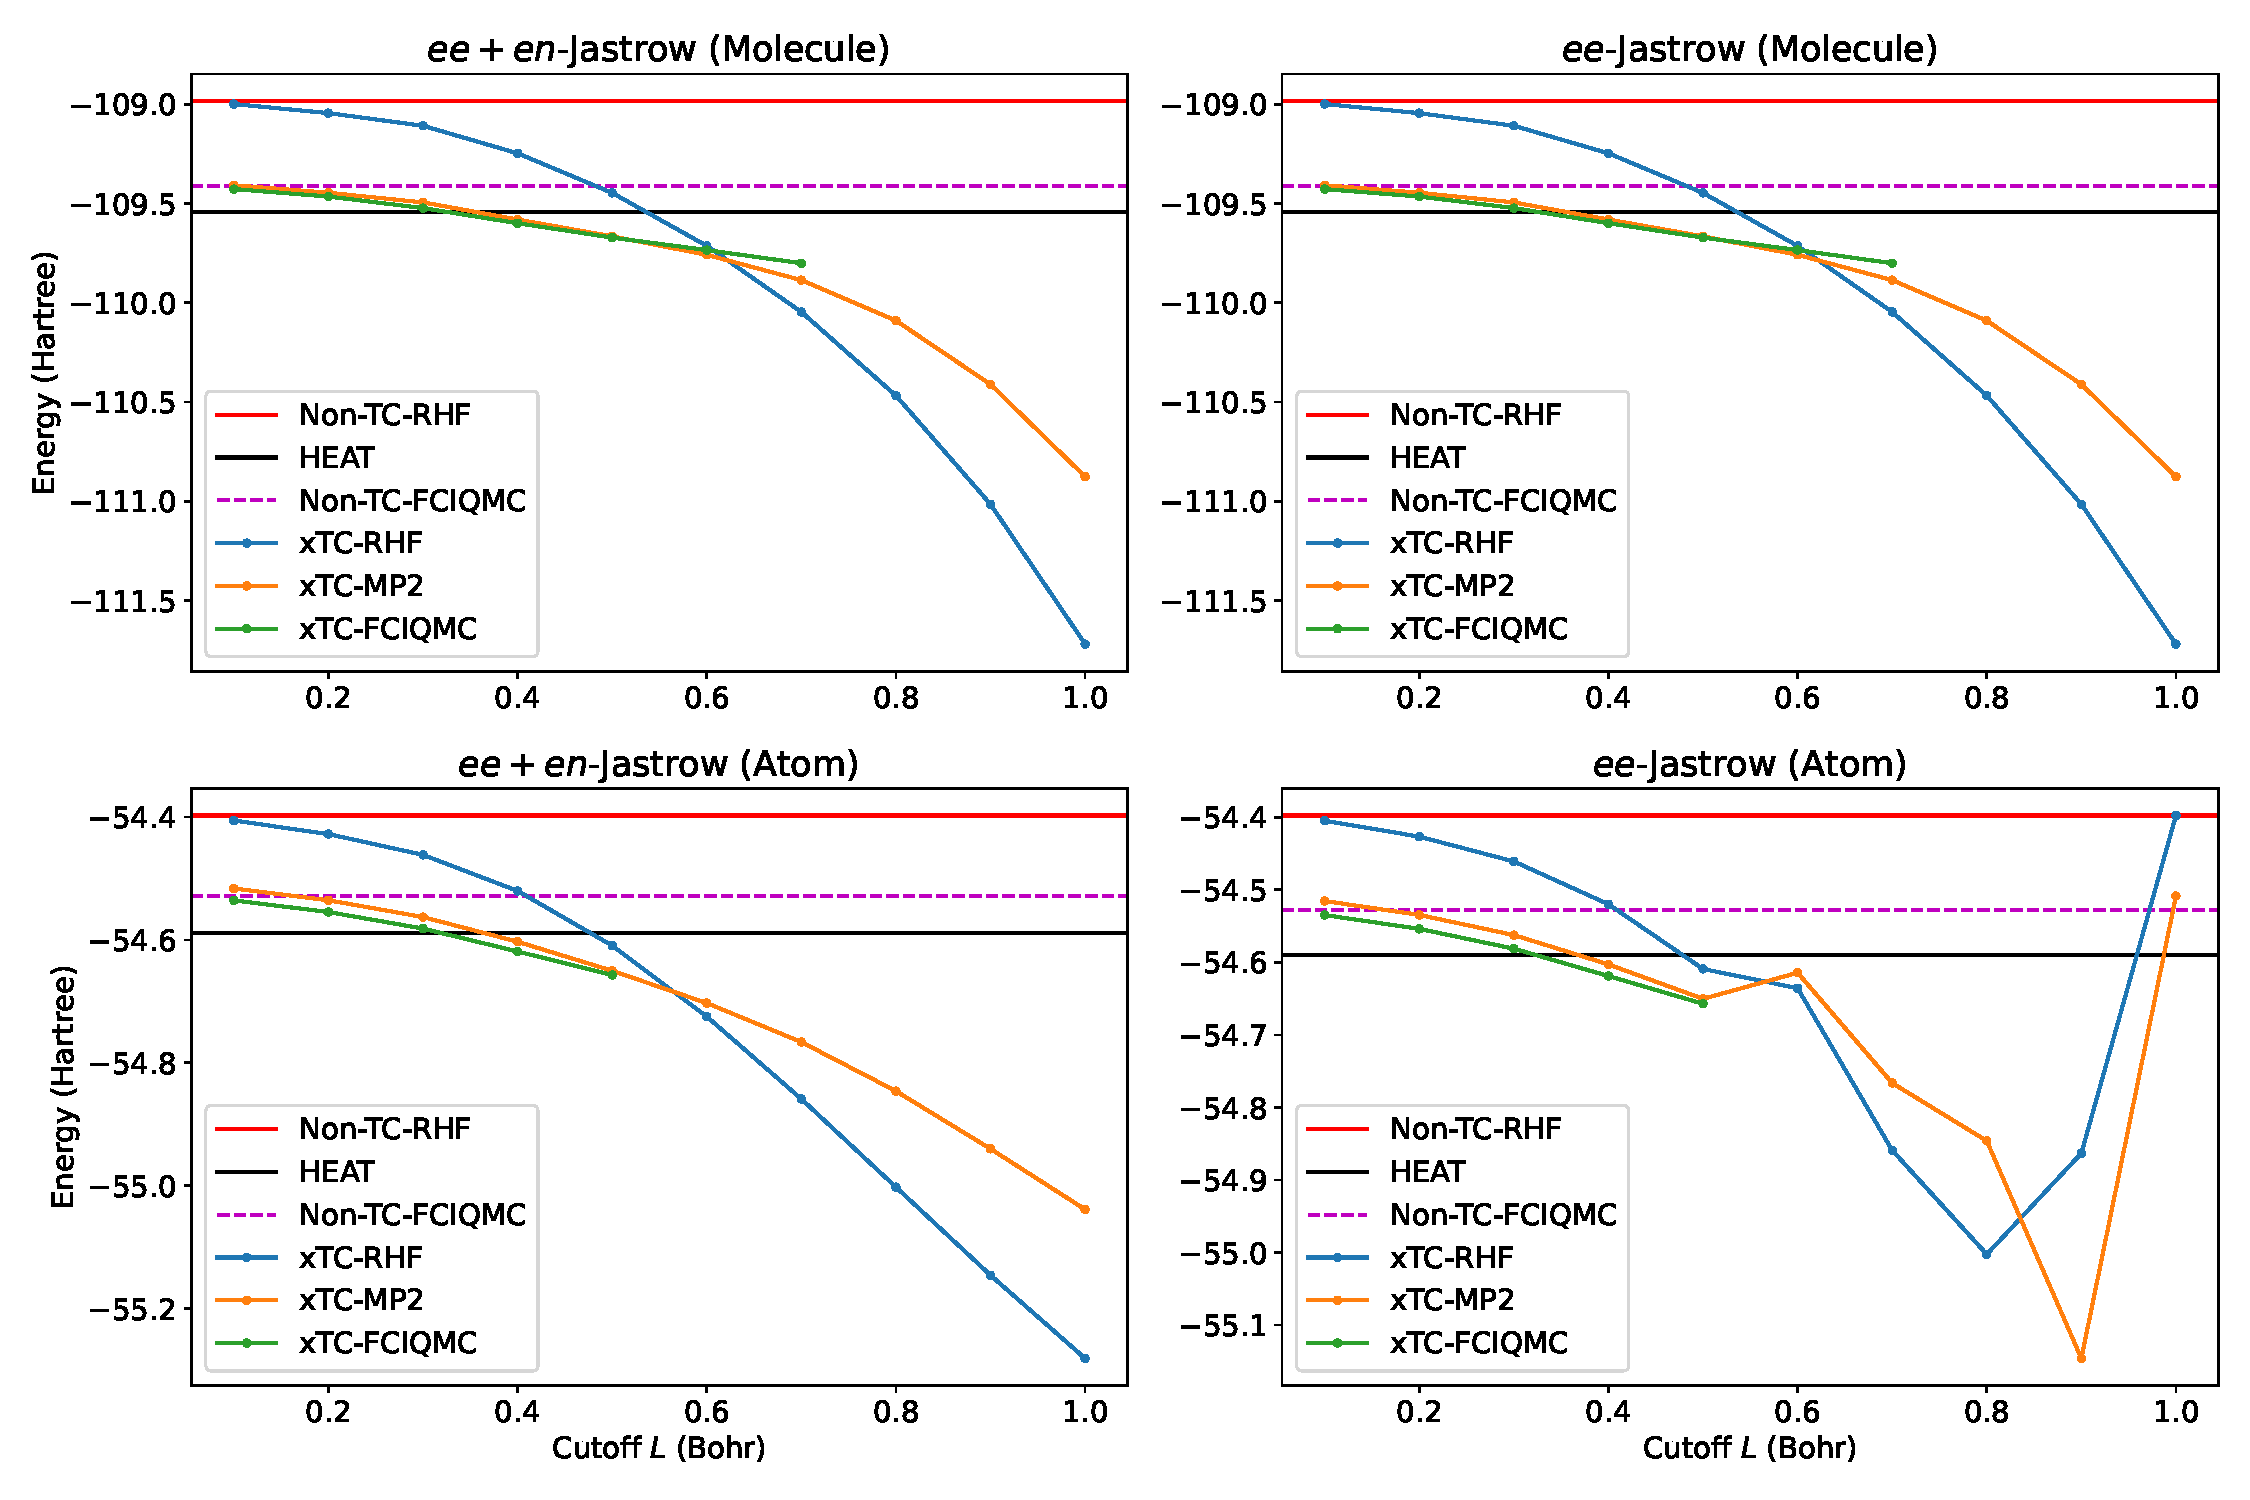
\includegraphics[width=\textwidth]{figures/universal/cutoffs_combined}
    \caption{Energy estimates for the nitrogen molecule (top panel) and atom (bottom panel) as a function of a cutoff parameter $L$ for the $ee+en$- (left panel) and $ee$-Jastrow (right panel) factors. The non-TC reference (RHF) energies are represented by a horizontal red line, the HEAT result by a horizontal black line, and the non-TC-FCIQMC by a dashed line. Since HEAT is a \gls{CBS}-extrapolated method, we wish for our TC energies to be above this value, while we also wish to improve upon the non-TC-FCIQMC energy. We therefore take the value of $L$ that leads to sensible energies (i.e. above the HEAT result), which is $L=0.3$ for all four plots. Large- and small-$L$ limits behave as expected, with the former giving nonsensical results and the former approximating the non-TC results in that basis set. All calculations were performed with the \avtz basis set. Missing xTC-FCIQMC points are due to numerical instability caused by a positive correlation energy. In practice, these may be resolved by setting a positive shift, but these results are anyway undesirable.}
    \label{fig:fournais-cutoff-n2}
\end{figure}

\subsection{Atomic Jastrow Factors}

Another approach we consider in reducing the need for optimisation is to optimise Jastrow factors for atomic systems and then reuse them in the molecular context. This can be considered a natural TC extension of starting with atomic orbitals for molecules. The key advantage here is flexibility while the key disadvantages include the need to optimise for the atoms, and the need to make a choice for the form of the Jastrow factor. In principle, we could produce a database of sophisticated atomic Jastrow factors that can then be queried to construct Jastrow factors for molecules or periodic systems. We use the Jastrow forms considered earlier in this dissertation, \begin{equation}
    \label{eq:jastrow-3}
    J = \sum_{i<j}^Nv(r_{ij}) + \sum_i^N\sum_I^{N_A}\chi(r_{iI}) + \sum_{i<j}^N\sum_I^{N_A}f(r_{ij}, r_{iI}, r_{jI}),
\end{equation}
with
\begin{equation}
    \label{eq:dtn-jastrow-ee-3}
    v(r_{ij})    = t(r_{ij},L_v)
                    \sum_{k} a_k r_{ij}^k ,
\end{equation}
\begin{equation}
    \label{eq:dtn-jastrow-en-3}
    \chi(r_{iI}) = t(r_{iI},L_\chi)
    \sum_{k} b_k r_{iI}^k ,
\end{equation}
\begin{equation}
    \label{eq:dtn-jastrow-een-3}
    f(r_{ij}, r_{i}, r_{j}) = t(r_{iI},L_f) t(r_{jI},L_f)
    \sum_{k,l,m} c_{klm}
    r_{ij}^k r_{iI}^l r_{jI}^m ,
\end{equation}
and the same cutoff functions $t(r,L) = (1-r/L)^3
\Theta(r-L)$. However, we do not want to include long-range (with respect to the nucleus) correlation in the atomic Jastrow factors, since this may bias the molecular calculations. We therefore use $L_v=L_\chi=1.0$ Bohr and $L_{v}=4.5$ Bohr. We consider the following variants:
\begin{itemize}
    \item The Jastrow factor is kept constant for the molecule, i.e. we simply use the atomic Jastrow factors as they are.
    \item We optimise the atomic Jastrow factor only with terms involving the nucleus, i.e. electron-nucleus and electron-electron-nucleus terms. The electron-electron part is then added to the atomic Jastrow and optimised for the molecule with the electron-nucleus and electron-electron-nucleus term fixed at the values determined for the atom. We optimise both with a single- and multideterminantal VMC ansatz.
\end{itemize}

We find these to yield results above HEAT and therefore do not concern ourselves with a cutoff analysis as in the case of the universal Jastrow factors.

\section{Results}

\subsection{Computational Details}

We revisit the nitrogen binding curve from \autoref{chap:binding} as a stress test for our Jastrow factors, as well as the atomisation of the molecules N$_2$, C$_2$, O$_2$, and CN from \autoref{chap:opt}. As before, we compare the results of the different choices of Jastrow factors against experiment\supercite{leroyAccurate2006} and the atomisation energies to HEAT.\supercite{fellerSurvey2008}

For the multideterminantal optimisation, we use a small FCIQMC calculation as it was found to perform particularly well in \autoref{chap:binding}, while keeping the orbitals consistent with the atom. Non-TC HF and CASCI calculations were performed using \pyscf,\supercite{sunPySCF2018} VMC optimisation was performed using \casino,\supercite{needsVariational2020} FCIQMC calculations using \neci,\supercite{gutherNECI2020} and MRCI-F12 calculations for comparison using \molpro.\supercite{wernerMOLPRO,wernerMolpro2012,wernerMolproQuantumChemistry2020}

\subsection{Binding Curves}
\todo{...}
\todo{universal Jastrows cutoff study -- also mention the pseudoMP2 values}

\subsection{Atomisation Energies}
\todo{...}

% \todo{N2 binding curve, some atomisation energies (I guess C2, N2 and CN are enough, say only with multidet(?) ee opt atom and en-ee universal)}

\section{Conclusion and Outlook}
\todo{mention the shortcoming of not being able to target specific states like the previous methodology (except for quasi-atomic)}
\todo{mention the fournais/universal form does not faithfully capture long-range correlation}
\todo{mention possibility of combining methods, also using the orbital cusp correction for the Fournais factor}
\todo{mention that with the small optimisation we introduce the possibility of targeting specific states, at least somewhat}
\todo{mention revisiting the universal Jastrow factors and the cutoffs more thoroughly}
\todo{...}

\todo{Also mention (maybe by then you even have data for) the Fournais Jastrow factor}
